%%%%%%%%%%%%%%%%%%%%%%%%%%%%%%%%%%%%%%%%%%%%%%%%
%%%%%%%%%%%%%%%%%%%%%%%%%%%%%%%%%%%%%%%%%%%%%%%%
\section{Prompt Templates for Annotation Tasks}
\label{apd:llm_prompts}

\subsection{LLM prompt to generate textual time-series from PMOA case reports}
\label{apd:extraction_prompt}

\begin{tcolorbox}[colback=gray!5, colframe=gray!100, title=Prompt, boxrule=2pt]
You are a physician. Extract the clinical events and the related time stamp from the case report. The admission event has timestamp 0. If the event is not available, we treat the event, e.g. current main clinical diagnosis or treatment with timestamp 0. The events that happened before event with 0 timestamp have negative time, the ones after the event with 0 timestamp have positive time. The timestamp are in hours. The unit will be omitted when output the result. If there is no temporal information of the event, please use your knowledge and events with temporal expression before and after the events to provide an approximation. We want to predict the future events given the events happened in history. For example, here is the case report.\\

\textcolor{teal}{\texttt{An 18-year-old male was admitted to the hospital with a 3-day history of fever and rash. Four weeks ago, he was diagnosed with acne and received the treatment with minocycline, 100 mg daily, for 3 weeks. With increased WBC count, eosinophilia, and systemic involvement, this patient was diagnosed with DRESS syndrome. The fever and rash persisted through admission, and diffuse erythematous or maculopapular eruption with pruritus was present. One day later the patient was discharged.}}\\

Let's find the locations of event in the case report, it shows that four weeks ago of fever and rash, four weeks ago, he was diagnosed with acne and receive treatment. So the event of fever and rash happened four weeks ago, 672 hours, it is before admitted to the hospital, so the time stamp is -672. diffuse erythematous or maculopapular eruption with pruritus was documented on the admission exam, so the timestamp is 0 hours, since it happens right at admission. DRESS syndrome has no specific time, but it should happen soon after admission to the hospital, so we use our clinical judgment to give the diagnosis of DRESS syndrome the timestamp 0. then the output should look like:\\

%\vspace{2mm}
\texttt{18 years old | 0 \\
male | 0 \\
admitted to the hospital | 0
fever | -72 \\
rash | -72 \\
acne | -672 \\
minocycline | -672 \\
increased WBC count | 0 \\
eosinophilia| 0 \\
systemic involvement| 0 \\
diffuse erythematous or maculopapular eruption| 0 \\
pruritis | 0 \\
DRESS syndrome | 0 \\
fever persisted | 0 \\
rash persisted | 0 \\
discharged | 24} \\

Separate conjunctive phrases into its component events and assign them the same timestamp (for example, separation of ‘fever and rash’ into 2 events: ‘fever’ and ‘rash’). If the event has duration, assign the event time as the start of the time interval. Attempt to use the text span without modifications except ‘history of’ where applicable. Include all patient events, even if they appear in the discussion; do not omit any events; include termination/discontinuation events; include the pertinent negative findings, like ‘no shortness of breath’ and ‘denies chest pain’. Show the events and timestamps in rows, each row has two columns: one column for the event, the other column for the timestamp. The time is a numeric value in hour unit. The two columns are separated by a pipe ‘|’ as a bar-separated file. Reply with the table only.
\end{tcolorbox}


%%%%%%%%%%%%%%%%%%%%%%%%%%%%%%%%%%%%%%%%%%%%%%%%
%%%%%%%%%%%%%%%%%%%%%%%%%%%%%%%%%%%%%%%%%%%%%%%%

%%\clearpage
\subsection{LLM prompt to extract demographics from PMOA case reports}
\label{apd:demographics_prompt}

\begin{tcolorbox}[colback=gray!5, colframe=gray!100, title=Prompt, boxrule=2pt]
You are an expert clinician. Extract the following demographic information from the case report: (1) age at case presentation, (2) sex (biologic sex at birth), and (3) ethnicity.  Report the age in years.  Report the sex as Male, Female, otherwise as a custom string, or Not Specified.  Report ethnicity as according to the US Census, otherwise as Not Specified.  For example, here is the case report.\\

\textcolor{teal}{\texttt{An 18-year-old male was admitted to the hospital with a 3-day history of fever and rash. Four weeks ago, he was diagnosed with acne and received the treatment with minocycline, 100 mg daily, for 3 weeks. With increased WBC count, eosinophilia, and systemic involvement, this patient was diagnosed with DRESS syndrome. The fever and rash persisted through admission, and diffuse erythematous or maculopapular eruption with pruritus was present. One day later the patient was discharged.}}\\

% \noindent
Then the demographic extraction should be:\\
\texttt{18 | Male | Not Specified} \\
 
Report the demographics with the three columns separated by a pipe '|' as a bar-separated row as above.
\end{tcolorbox}

%%%%%%%%%%%%%%%%%%%%%%%%%%%%%%%%%%%%%%%%%%%%%%%%
%%%%%%%%%%%%%%%%%%%%%%%%%%%%%%%%%%%%%%%%%%%%%%%%

%%\clearpage
\subsection{LLM prompt to extract list of diagnoses from PMOA case reports}
\label{apd:diagnosis_prompt}

\begin{tcolorbox}[colback=gray!5, colframe=gray!100, title=Prompt, boxrule=2pt]
You are an expert physician.  Output the list of diagnoses that pertain to the patient in the case report. For example, here is the case report.\\

\textcolor{teal}{\texttt{An 18-year-old male was admitted to the hospital with a 3-day history of fever and rash. Four weeks ago, he was diagnosed with acne and received the treatment with minocycline, 100 mg daily, for 3 weeks. With increased WBC count, eosinophilia, and systemic involvement, this patient was diagnosed with DRESS syndrome. The fever and rash persisted through admission and diffuse erythematous or maculopapular eruption with pruritus was present. One day later the patient was discharged.}} \\

Then the output should look like:\\
    \texttt{acne} \\
    \texttt{DRESS syndrome} \\

Rash, leukocytosis, and other findings are not diseases so they are omitted, while acne and DRESS syndrome were both diagnosed, so they are included. Output a list of diagnoses (one per line) from the following case. Place the primary diagnosis first. Include only the list and nothing else.

\end{tcolorbox}


%%%%%%%%%%%%%%%%%%%%%%%%%%%%%%%%%%%%%%%%%%%%%%%%
%%%%%%%%%%%%%%%%%%%%%%%%%%%%%%%%%%%%%%%%%%%%%%%%

%\clearpage
\section{Comparing LLM Annotations}
\label{apd:example_annotations}

In this section, we showcase an excerpt from PMC10629858, the latest case included in the sepsis-10 dataset \citep{abu2023rare}. To demonstrate the extraction task and analyze the performance of various LLM annotators, we compare manual annotations against outputs from several LLM variants: DeepSeek-R1, DeepSeek-R1-UD-IQ1, DeepSeek-V3-0324, LLaMA 3.3 70B, OpenAI O1, OpenAI O3, and OpenAI O4-mini.

\newcolumntype{P}[1]{>{\raggedright\hangindent=1em\hangafter=1}p{#1}}
\begin{figure*}[t]
    Excerpt from \cite{abu2023rare}:
    \begin{quote}\footnotesize
    A 57-year-old man recently diagnosed with lepromatous leprosy was confirmed with skin biopsy and had been on treatment (rifampicin/clofazimine/dapsone) for 2 months before admission; he was presented to the hospital with complaints of abdominal distension, constipation, vomiting, and a 10-kg weight loss. On examination, the patient was vitally stable. He had evidence of peripheral lymphadenopathy with a distended abdomen and a positive shifting dullness. A computed tomography scan of his abdomen showed mural thickening of the terminal ileum with significantly enlarged mesenteric lymph nodes, mesenteric fat stranding, and intra-abdominal free fluid, suggesting abdominal granulomatous infection or neoplastic process.
    \dots 
    
    The patient was planned for consolidation by autologous bone marrow transplant. Unfortunately, with the recurrent bacteremia and sepsis that accompanied the patient’s course due to his immunocompromised state, he was re-admitted to the medical ICU for severe sepsis and multiorgan failure and passed away around 6 months after his initial diagnosis with NHL, despite maintaining a remission status.
    \end{quote}

    % DeepSeek-R1, DeepSeek-R1-UD-IQ1, DeepSeek-V3-
    % 0324, LLaMA 3.3 70B, OpenAI O1, OpenAI O3, and OpenAI O4-mini

    %%%%%%%%%%%%%%%%%%%%%%%%%%%%%%%%%%%%%%%%%%%%%%%%%%%%%%%%
    %%%%%%%% Manual and DeepSeek R1 %%%%%%%%%%%%%%%%%%%%%%%%%%%%%%
    %%%%%%%%%%%%%%%%%%%%%%%%%%%%%%%%%%%%%%%%%%%%%%%%%%%%%%%%

    \begin{minipage}[!htbp]{0.49\textwidth}
    \footnotesize
        \textbf{Manual annotation} \\ \\
        \footnotesize
        \begin{tabular}{P{0.75\textwidth}r}
            57-year-old&0 \\
            man&0 \\
            diagnosed with lepromatous leprosy&-1461 \\
            on treatment&-1461 \\
            rifampicin&-1461 \\
            clofazimine&-1461 \\
            dapsone&-1461 \\
            presented to the hospital&0 \\
            abdominal distension&0 \\
            constipation&0 \\
            vomiting&0 \\
            10-kg weight loss&0 \\
            vitally stable&0 \\
            peripheral lymphadenopathy&0 \\
            distended abdomen&0 \\
            positive shifting dullness&0 \\
            computed tomography scan of his abdomen&0 \\
            mural thickening of the terminal ileum&0 \\
            significantly enlarged mesenteric lymph nodes&0 \\
            mesenteric fat stranding&0 \\
            intra-abdominal free fluid&0 \\
            % Abdominal paracentesis&0 \\
            re-admitted to the medical ICU&4383 \\
            severe sepsis&4383 \\
            multiorgan failure&4383 \\
            passed away&4383
        \end{tabular}
    \end{minipage}
    \begin{minipage}[!htbp]{0.49\textwidth}
    \footnotesize
        \textbf{DeepSeek-R1 annotation} \\ \\
        \footnotesize
        \begin{tabular}{P{0.75\textwidth}r}
            57 years old & 0 \\
            male & 0 \\
            lepromatous leprosy & -1464 \\
            skin biopsy & -1464 \\
            rifampicin & -1464 \\
            clofazimine & -1464 \\
            dapsone & -1464 \\
            admitted to the hospital & 0 \\
            abdominal distension & 0 \\
            constipation & 0 \\
            vomiting & 0 \\
            10-kg weight loss & 0 \\
            vital stability & 0 \\
            peripheral lymphadenopathy & 0 \\
            distended abdomen & 0 \\
            positive shifting dullness & 0 \\
            computed tomography scan & 0 \\
            mural thickening of the terminal ileum & 0 \\
            enlarged mesenteric lymph nodes & 0 \\
            mesenteric fat stranding & 0 \\
            intra-abdominal free fluid & 0 \\
            abdominal paracentesis & 0 \\
            plan for autologous bone marrow transplant & 4320 \\
            recurrent bacteremia & 4320 \\
            sepsis & 4320 \\
            readmission to ICU & 4320 \\
            severe sepsis & 4320 \\
            multiorgan failure & 4320 \\
            death & 4320 \\
            & 
        \end{tabular}
    \end{minipage}

\end{figure*}

%%%%%%%%%%%%%%%%%%%%%%%%%%%%%%%%%%%%%%%%%%%%%%%%%%%%%%%%
%%%%%%%%  DeepSeek-V3 and Llama 3.3 70B %%%%%%
%%%%%%%%%%%%%%%%%%%%%%%%%%%%%%%%%%%%%%%%%%%%%%%%%%%%%%%%
\begin{figure*}[!htbp]
    \begin{minipage}[!htbp]{0.49\textwidth}
    \footnotesize
        \textbf{DeepSeek-V3-0324 annotation} \\ \\
        \footnotesize
        \begin{tabular}{P{0.75\textwidth}r}
            57 years old & 0 \\
            male & 0 \\
            lepromatous leprosy & -1464 \\
            skin biopsy & -1464 \\
            rifampicin & -1464 \\
            clofazimine & -1464 \\
            dapsone & -1464 \\
            admitted to the hospital & 0 \\
            abdominal distension & 0 \\
            constipation & 0 \\
            vomiting & 0 \\
            weight loss & 0 \\
            peripheral lymphadenopathy & 0 \\
            distended abdomen & 0 \\
            positive shifting dullness & 0 \\
            computed tomography scan & 0 \\
            mural thickening of the terminal ileum & 0 \\
            enlarged mesenteric lymph nodes & 0 \\
            mesenteric fat stranding & 0 \\
            intra-abdominal free fluid & 0 \\
            abdominal granulomatous infection & 0 \\
            neoplastic process & 0 \\
            abdominal paracentesis & 0 \\
            autologous bone marrow transplant planned & 672 \\
            recurrent bacteremia & 672 \\
            sepsis & 672 \\
            re-admitted to the medical ICU & 4032 \\
            severe sepsis & 4032 \\
            multiorgan failure & 4032 \\
            passed away & 4032 \\
            complete metabolic remission & 4032 \\
        \end{tabular}
    \end{minipage}
    \begin{minipage}[!htbp]{0.49\textwidth}
    \footnotesize
        \textbf{LLaMA 3.3 70B annotation} \\ \\
        \footnotesize
        \begin{tabular}{P{0.75\textwidth}r}
            57 years old & 0 \\
            male & 0 \\
            lepromatous leprosy & -144 \\
            skin biopsy & -144 \\
            rifampicin & -144 \\
            clofazimine & -144 \\
            dapsone & -144 \\
            abdominal distension & 0 \\
            constipation & 0 \\
            vomiting & 0 \\
            weight loss & 0 \\
            peripheral lymphadenopathy & 0 \\
            distended abdomen & 0 \\
            positive shifting dullness & 0 \\
            mural thickening of the terminal ileum & 0 \\
            enlarged mesenteric lymph nodes & 0 \\
            mesenteric fat stranding & 0 \\
            intra-abdominal free fluid & 0 \\
            abdominal granulomatous infection & 0 \\
            neoplastic process & 0 \\
            autologous bone marrow transplant & 1344 \\
            recurrent bacteremia & 1344 \\
            sepsis & 1344 \\
            multiorgan failure & 1344 \\
            passed away & 1440 \\
            & 
        \end{tabular}
    \end{minipage}
\end{figure*}
%%%%%%%%%%%%%%%%%%%%%%%%%%%%%%%%%%%%%%%%%%%%%%%%%%%%%%%%
%%%%%%%% GPT5 and O1 %%%%%%%%%%%%%%%%%%%%%%%%%%%%%%
%%%%%%%%%%%%%%%%%%%%%%%%%%%%%%%%%%%%%%%%%%%%%%%%%%%%%%%%
\begin{figure*}[!htbp]
    \begin{minipage}[!htbp]{0.49\textwidth}
    \footnotesize
        \textbf{GPT5 annotation} \\ \\
        \footnotesize
        \begin{tabular}{P{0.75\textwidth}r}
            57-year-old man & 0 \\
            male & 0 \\
            recently diagnosed with lepromatous leprosy & -1440 \\
            skin biopsy confirmed lepromatous leprosy & -1440 \\
            rifampicin started & -1440 \\
            clofazimine started & -1440 \\
            dapsone started & -1440 \\
            presented to the hospital with complaints of abdominal distension & 0 \\
            constipation & 0 \\
            vomiting & 0 \\
            10-kg weight loss & 0 \\
            peripheral lymphadenopathy & 0 \\
            distended abdomen & 0 \\
            positive shifting dullness & 0 \\
            computed tomography scan of his abdomen & 6\\
            mural thickening of the terminal ileum & 6 \\
            significantly enlarged mesenteric lymph nodes & 6 \\
            mesenteric fat stranding & 6 \\
            intra-abdominal free fluid & 6 \\
            abdominal granulomatous infection or neoplastic process suggested & 6 \\
            abdominal paracentesis was done & 6 \\
            recurrent bacteremia & 1200 \\
            % neoplastic process & 0 \\
            planned for consolidation by autologous bone marrow transplant & 2400 \\
            remission status maintained & 4200 \\
            re-admitted to the medical ICU for severe sepsis and multiorgan failure & 4296 \\
            passed away & 4320 \\
        \end{tabular}
    \end{minipage}
    \begin{minipage}[!htbp]{0.49\textwidth}
    \footnotesize
        \textbf{OpenAI O1 annotation} \\ \\
        \footnotesize
        \begin{tabular}{P{0.75\textwidth}r}
            % 57 years old & -1440 \\
            % male & -1440 \\
            diagnosed with lepromatous leprosy & -1344 \\  
            confirmed with skin biopsy & -1344 \\  
            treatment with rifampicin/clofazimine/dapsone & -1344 \\  
            admitted to the hospital & 0 \\ 
            vitally stable & 0 \\
            abdominal distension & 0 \\  
            constipation & 0 \\  
            vomiting & 0 \\ 
            10-kg weight loss & 0 \\   
            peripheral lymphadenopathy & 0 \\  
            distended abdomen & 0 \\  
            positive shifting dullness & 0 \\  
            computed tomography scan & 0 \\  
            mural thickening of the terminal ileum & 0 \\  
            significantly enlarged mesenteric lymph nodes & 0 \\  
            mesenteric fat stranding & 0 \\  
            intra-abdominal free fluid & 0 \\  
            suggesting abdominal granulomatous infection or neoplastic process & 0 \\  
            abdominal paracentesis & 0 \\ 
            % Planned for consolidation by autologous bone marrow transplant & 2136  \\
            % Responded well to chemotherapy & 2280   \\
            % Attained complete metabolic remission by positron emission tomography/computed tomography & 2280   \\
            planned for consolidation by autologous bone marrow transplant & 2500 \\  
            re-admitted to the medical ICU  & 3000 \\  
            severe sepsis &	3000 \\
            multiorgan failure & 3000 \\
            passed away & 4320 \\
            & 
        \end{tabular}
    \end{minipage}
\end{figure*} 

%%%%%%%%%%%%%%%%%%%%%%%%%%%%%%%%%%%%%%%%%%%%%%%%%%%%%%%%
%%%%%%%% O3 and O4-mini %%%%%%%%%%%%%%%%%%%%%%%%%%%%%%
%%%%%%%%%%%%%%%%%%%%%%%%%%%%%%%%%%%%%%%%%%%%%%%%%%%%%%%%
\begin{figure*}[!htbp]
    \begin{minipage}[!htbp]{0.49\textwidth}
    \footnotesize
        \textbf{OpenAI O3 annotation} \\ \\
        \footnotesize
        \begin{tabular}{P{0.75\textwidth}r}
            lepromatous leprosy diagnosis & -1440 \\
            skin biopsy confirmed lepromatous leprosy & -1440 \\
            rifampicin treatment started & -1440 \\
            clofazimine treatment started & -1440 \\
            dapsone treatment started & -1440 \\
            presented to hospital & 0 \\
            abdominal distension & 0 \\
            constipation & 0 \\
            vomiting & 0 \\
            10-kg weight loss & 0 \\
            vitally stable & 0 \\
            peripheral lymphadenopathy & 0 \\
            distended abdomen & 0 \\
            positive shifting dullness & 0 \\
            computed tomography abdomen & 0 \\
            mural thickening of terminal ileum & 0 \\
            enlarged mesenteric lymph nodes & 0 \\
            mesenteric fat stranding & 0 \\
            intra-abdominal free fluid & 0 \\
            abdominal granulomatous infection suggested & 0 \\
            neoplastic process suggested & 0 \\
            abdominal paracentesis & 0 \\
            planned autologous bone marrow transplant & 2150 \\
            % assessment after four cycles & 2208 \\
            % complete metabolic remission on PET/CT & 2208 \\
            re‑admission to medical ICU & 4320 \\
            severe sepsis & 4320 \\
            multiorgan failure & 4320 \\
            death & 4320 \\
            remission status maintained & 4320
        \end{tabular}
    \end{minipage}
    \begin{minipage}[!htbp]{0.49\textwidth}
    \footnotesize
        \textbf{OpenAI O4-mini annotation} \\ \\
        \footnotesize
        \begin{tabular}{P{0.75\textwidth}r}
            lepromatous leprosy confirmed with skin biopsy & -1440 \\  
            rifampicin treatment started & -1440 \\  
            clofazimine treatment started & -1440 \\  
            dapsone treatment started & -1440 \\  
            57 years old & 0 \\  
            male & 0 \\ 
            presented to the hospital & 0 \\  
            complaint of abdominal distension & 0 \\  
            complaint of constipation & 0 \\  
            complaint of vomiting & 0 \\  
            10-kg weight loss & 0 \\  
            vitals stable & 0 \\  
            peripheral lymphadenopathy & 0 \\  
            distended abdomen & 0 \\  
            positive shifting dullness & 0 \\  
            mural thickening of the terminal ileum & 0 \\  
            significantly enlarged mesenteric lymph nodes & 0 \\  
            mesenteric fat stranding & 0 \\  
            intra-abdominal free fluid & 0 \\  
            abdominal paracentesis performed & 2 \\ 
            plan autologous bone marrow transplant & 1900 \\  
            %assessment after four cycles of EPOCH & 2256 \\  
            % response to chemotherapy achieved & 2256 \\  
            % complete metabolic remission attained by PET/CT &2256 \\  
            re-admission to medical ICU for severe sepsis and multiorgan failure & 4260 \\
            death & 4320 \\
            & 
        \end{tabular}
    \end{minipage}
    \caption{TTS comparison across multiple LLMs}
    \label{fig:compare_LLM_annotations}
\end{figure*}




%%%%%%%%%%%%%%%%%%%%%%%%%%%%%%%%%%%%%%%%%%%%%%%%
%%%%%%%%%%%%%%%%%%%%%%%%%%%%%%%%%%%%%%%%%%%%%%%%
%\clearpage
\section{Log-Time Cumulative Distribution Function}
\label{apd:ltcdf}
Recall the log-time cumulative distribution function is given as follows:
\[
   F(x) = \frac{1}{k} \sum_{i=1}^k \mathds{1}\{\{x_{(i)} \leq x\}\},
\]
where $\mathds{1}$ is the indicator function.

We compute the AULTC as the area under $F(x)$ from $x = 0$ to $x = \log(1 + S_{\text{max}})$, normalized by $\log(1 + S_{\text{max}})$:
\begin{align*}
\text{AULTC} &= \frac{1}{\log(1 + S_{\text{max}})} \Bigg[ \sum_{i=1}^k (x_{(i)} - x_{(i-1)}) \frac{i}{k} + (\log(1 + S_{\text{max}}) - x_{(k)}) \times 1 \Bigg]
\end{align*}
where $x_{(0)} = 0$. With this definition, AULTC = 1 indicates that discrepancies are zero (perfect recovery), resulting in maximum area $\log(1 + S_{\text{max}})$, and AULTC = 0 indicates that all discrepancies exceed $S_{\text{max}}$, yielding zero area. 
% The code for the AULTC calculation is given in the function \texttt{ecdf\textunderscore auc2(\dots)} in the Supplementary Materials.


\begin{remark}
The time unit and cutoff $S_\text{max}$ affect the AULTC calculation, so they must be specified when reporting the AULTC.
\end{remark}

Because of the $\log(1 + \cdot)$ transformation (rather than the $\log(\cdot)$ transformation which is undefined for zero time-error discrepancy), the discrepancies are non-linearly shifted in the log scale.  The non-linear shift adjusts the relative widths of the step function (particularly for small discrepancies) changing the area calculation.  The cutoff $S_\text{max}$ affects the normalization factor.  Therefore, these values should be chosen based on practicalities for the application.  In our case, we chose hours at the time unit because the only sub-hour descriptions reported were several Apgar scores at the minute-level.

\begin{remark}
    The average log-time discrepancy is non-convex.
\end{remark}
This can be seen from the observation that the $\log(1+\cdot)$ function is ``spikier'' than the L1 function. More formally, the log-time discrepancy has a higher curvature around zero error compared to the L1 loss. Consider the second derivatives of the loss functions with respect to the discrepancies $s = |t^p - t^r|$.  For L1 loss $L_1(s) = s$, the second derivative $\frac{d^2 L_1}{ds^2} = 0$ for $s > 0$.
For the log-time loss, $L_{log}(s) = \log(1 + s)$, the second derivative is $\frac{d^2 L_{log}}{ds^2} = -\frac{1}{(1 + s)^2}$. At $s = 0$, the second derivative is $-1$, while the second derivative of the L1 loss is $0$.

To provide a simple counterexample, define the average log-time discrepancy is given by:
\[
L(t^p) = \frac{1}{k} \sum_{i=1}^k \log(1 + \min(|t^p_i - t^r_i|, S_{\text{max}}))
\]
To prove that this function is non-convex, we need to show that there exist $t^{p1}, t^{p2}$ and $\lambda \in (0,1)$ such that
\[
L(\lambda t^{p1} + (1-\lambda) t^{p2}) > \lambda L(t^{p1}) + (1-\lambda) L(t^{p2})
\]
Consider the case where $k=1$, $t^r = 0$, and $S_{\text{max}} = 2$. The loss function is $L(t^p) = \log(1 + \min(|t^p|, 2))$.
Let $t^{p1} = 0$ and $t^{p2} = 3$. Choose $\lambda = 0.5$.
Then $\lambda t^{p1} + (1-\lambda) t^{p2} = 0.5 \times 0 + 0.5 \times 3 = 1.5$.
Now we evaluate the loss function at these points:
\begin{align*}
L(t^{p1}) &= L(0) = \log(1 + \min(|0|, 2)) = 0 \\
L(t^{p2}) &= L(3) = \log(1 + \min(|3|, 2)) = \\
    & \qquad \log(3) \\
L(\lambda t^{p1} + (1-\lambda) t^{p2}) &= L(1.5) = \log(2.5)
\end{align*}
Now we check the convexity condition:
\[
L(1.5) \leq 0.5 L(0) + 0.5 L(3)
\]
\[
\log(2.5) \leq 0.5 \times 0 + 0.5 \times \log(3)
\]
\[
\log(2.5) \leq \log(\sqrt{3})
\]
Since $2.5 > \sqrt{3} \approx 1.732$, we have $\log(2.5) > \log(\sqrt{3})$.
Therefore,
\[
L(\lambda t^{p1} + (1-\lambda) t^{p2}) > \lambda L(t^{p1}) + (1-\lambda) L(t^{p2})
\]
This proves that the average log-time discrepancy is non-convex.
This remark illustrates the loss form, in case it is considered for optimization/model training rather than for assessment purposes.

%%%%%%%%%%%%%%%%%%%%%%%%%%%%%%%%%%%%%%%%%%%%%%%%
%%%%%%%%%%%%%%%%%%%%%%%%%%%%%%%%%%%%%%%%%%%%%%%%
%%\clearpage
\section{Recursive Best Match Procedure}
\label{apd:recursive_match}
We provide pseudocode for the best match procedure between two lists of strings (Algorithm \ref{alg:recursive_match}).  For each list, we use the text order, \emph{i.e.}, the order of the events in the annotation files, to break embedding distance ties.  We use the cosine similarity for the distance calculation using sentence transformer embeddings from \texttt{S-PubMedBert-MS-MARCO}.

\begin{algorithm}[ht]
\caption{Recursive Best Match}
\label{alg:recursive_match}
\begin{algorithmic}[1]
\Require Two lists: \texttt{ref} (reference events) and \texttt{pred} (predicted events)
\Ensure List of best-matching event pairs
\Function{MatchEvents}{\texttt{ref}, \texttt{pred}}
    \If{\texttt{ref} is empty \textbf{or} \texttt{pred} is empty}
        \State \Return $[]$
    \EndIf
    \State $\text{min\_distance} \gets \infty$
    \State $\text{best\_pair} \gets \text{None}$
    \ForAll{$r \in \texttt{ref}$}
        \ForAll{$p \in \texttt{pred}$}
            \State $d \gets \text{ComputeDistance}(r, p)$
            \If{$d < \text{min\_distance}$}
                \State $\text{min\_distance} \gets d$
                \State $\text{best\_pair} \gets (r, p)$
            \ElsIf{$d = \text{min\_distance}$}
                \State Get indices of $r$, $p$, and current $\text{best\_pair}$
                \If{index of $r <$ best $r$ index}
                    \State $\text{best\_pair} \gets (r, p)$
                \ElsIf{index of $r = $ best $r$ index \textbf{and} index of $p <$ best $p$ index}
                    \State $\text{best\_pair} \gets (r, p)$
                \EndIf
            \EndIf
        \EndFor
    \EndFor
    \State Remove $\text{best\_pair.r}$ from \texttt{ref}
    \State Remove $\text{best\_pair.p}$ from \texttt{pred}
    \State $\text{result} \gets [\text{best\_pair}] + \text{MatchEvents}(\texttt{ref}, \texttt{pred})$
    \State \Return $\text{result}$
\EndFunction
\end{algorithmic}
\end{algorithm}

%%%%%%%%%%%%%%%%%%%%%%%%%%%%%%%%%%%%%%%%%%%%%%%%
%%%%%%%%%%%%%%%%%%%%%%%%%%%%%%%%%%%%%%%%%%%%%%%%
%%\clearpage
\section{Varying the Event Match Distance Threshold}
\label{apd:choosing_match_threshold}

By varying the event match distance threshold, we obtain different performance characteristics for event match rate, event concordance, and temporal discrepancy (AULTC).  We choose a cosine similarity of 0.1 based on manual review of Llama 3.3 70B Instruct and o1 annotations.  Plotting the event match rate versus temporal performance characteristic (concordance and AULTC) when varying the threshold from 0.01 to 0.25, we obtain performance tradeoffs in Figure \ref{fig:threshold_temporal_tradeoff}.

\begin{figure}
    \centering
    \begin{minipage}{0.45\textwidth}
        \centering
        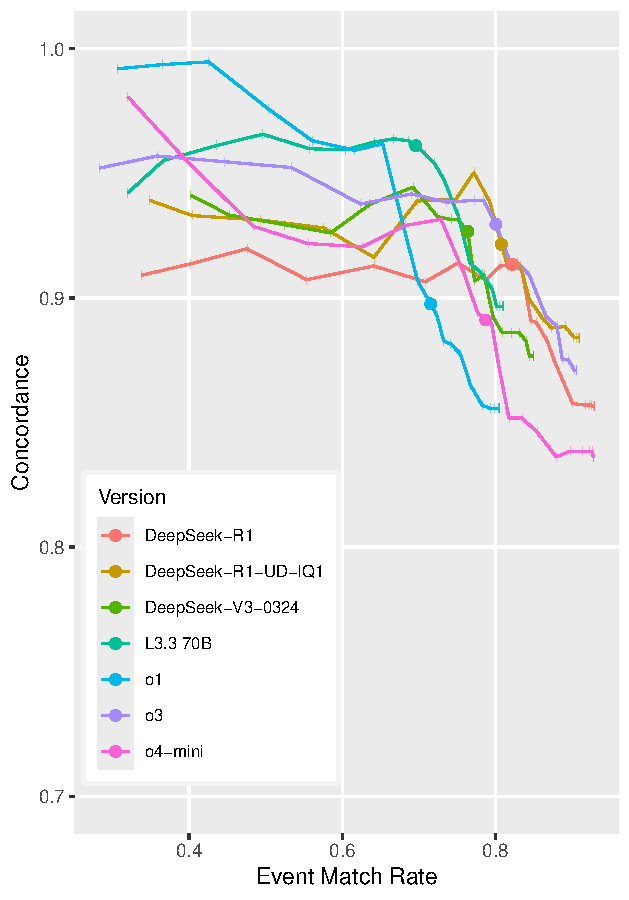
\includegraphics[width=\linewidth]{Plots_tables/match_threshold_concordance_plot.pdf}
        % \caption{}
    \end{minipage}
    % \hfill
    \begin{minipage}{0.45\textwidth}
        \centering
        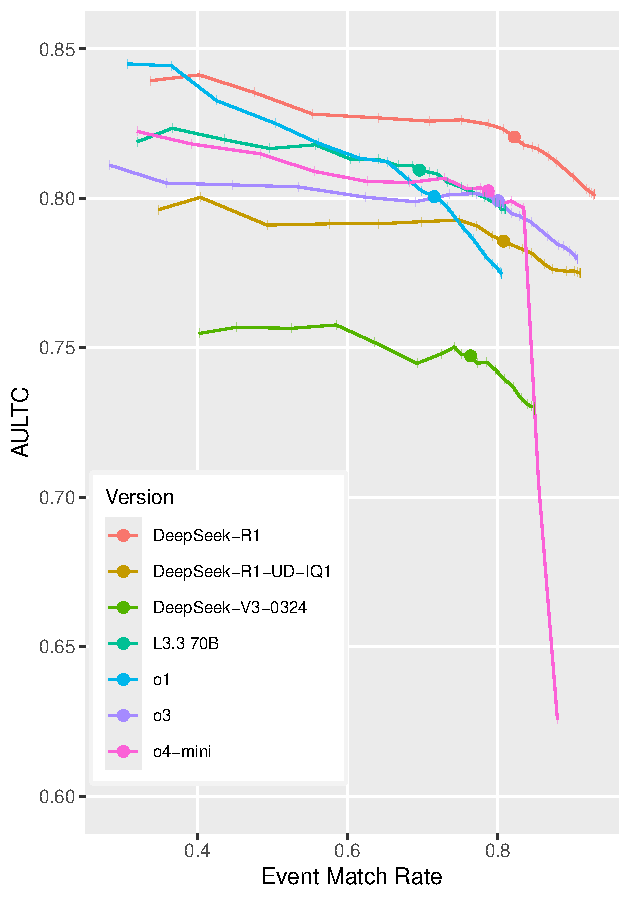
\includegraphics[width=\linewidth]{Plots_tables/match_threshold_plot.pdf}
        % \caption{}
    \end{minipage}
    \caption{\textbf{Left:} Concordance by event match rate. Solid circle ($\bullet$) represents threshold of 0.1, with ticks (|) indicating 0.01 increments of the threshold in [0.01, 0.25]. \textbf{Right:} AULTC by event match rate.}
    \label{fig:threshold_temporal_tradeoff}
\end{figure}

%%%%%%%%%%%%%%%%%%%%%%%%%%%%%%%%%%%%%%%%%%%%%%%%
%%%%%%%%%%%%%%%%%%%%%%%%%%%%%%%%%%%%%%%%%%%%%%%%
%%\clearpage
\section{UMLS Mapping for Diagnosis Standardization}
\label{apd:umls_mapping}

To standardize the diagnoses extracted by LLMs from the case reports, we mapped the free-text diagnoses to concepts in the Unified Medical Language System (UMLS). 
This process involved the following steps:

\begin{enumerate}
    \item \textbf{Initial Extraction}: For each case report, we prompted the LLM to extract diagnoses as described in Appendix \ref{apd:diagnosis_prompt}. 
    This yielded a list of free-text diagnoses for each case report.
    \item \textbf{Entity Linking}: We used ScispaCy's entity linker model 
    \texttt{(en\_core\_sci\_lg)} with the UMLS knowledge base to map each extracted diagnosis to corresponding UMLS Concept Unique Identifiers (CUIs). 
    The entity linker identifies potential UMLS concepts and ranks them based on contextual relevance.
    \item \textbf{Filtering and Disambiguation}: For each diagnosis, we:
    \begin{itemize}
       \item Retained only mappings with a confidence score above 0.85
       \item When multiple CUIs were identified for a single diagnosis, selected the highest-ranked mapping
    \end{itemize}
    \item \textbf{Concept Normalization}: After mapping to CUIs, we:
\begin{itemize}
   \item Retrieved the canonical names from UMLS Metathesaurus
   % \item Applied semantic type filtering to ensure mapped concepts were of types relevant to diagnoses (e.g., "Disease or Syndrome", "Pathologic Function", "Mental or Behavioral Dysfunction")
   % \item Grouped synonym concepts where appropriate to reduce redundancy
\end{itemize}
\end{enumerate}


This mapping process allowed us to standardize the diverse expressions of diagnoses extracted by LLMs into a consistent terminology system, enabling more reliable frequency analysis and co-occurrence patterns. 
% For diagnoses where high-confidence UMLS mapping was not achieved, we retained the original LLM-extracted text but flagged these entries in our analysis.

% The mapping was performed on a sample of 25,000 case reports, resulting in approximately 93,000 diagnosis instances mapped to 7,800 unique UMLS concepts.


%%%%%%%%%%%%%%%%%%%%%%%%%%%%%%%%%%%%%%%%%%%%%%%%
%%%%%%%%%%%%%%%%%%%%%%%%%%%%%%%%%%%%%%%%%%%%%%%%
%\clearpage

\section{Survival Analysis Task on PMOA-TTS}
\label{apd:survival_analysis}

We developed a survival analysis framework to evaluate the prognostic value of textual information encoded in the time series for time until death prediction. 
Our approach follows a two-stage process:

\begin{enumerate}[leftmargin=*,topsep=0pt,itemsep=0pt]
\item \textbf{Embedding Extraction}: Each textual time series is converted to a textual context in the format \texttt{"(time) clinical event [SEP] ... [SEP] (time) clinical event [SEP]"} and processed using various pre-trained language models to obtain dense vector representations. 
For encoder models (BERT, RoBERTa, ModernBERT, etc.), we extract the \texttt{[CLS]} token embedding, while for decoder models (LLaMA, DeepSeek), we compute the mean-pooled embedding over all non-padding tokens.

\item \textbf{Survival Modeling}: These embeddings serve as covariates for two survival models:
\begin{itemize}[leftmargin=*,topsep=0pt,itemsep=0pt]
    \item \textbf{DeepSurv} \citep{katzman2018deepsurv}: A neural network generalization of the Cox proportional hazards model.
    \item \textbf{DeepHit} \citep{lee2018deephit}: A multi-task neural network jointly modeling discrete hazard and survival functions.
\end{itemize}
\end{enumerate}

We evaluated the performance of the survival models using two metrics: the time-dependent concordance index \citep{antolini2005time}, which measures the model’s ability to correctly rank survival times, and the integrated Brier score (IBS), which captures overall calibration and discrimination over time. 

To ensure reliable estimates, we conducted experiments across five random seeds.
For each seed, we performed a train-validation-test split with proportions of 64\%, 16\%, and 20\%, respectively. 

All survival times were right-censored at a fixed cutoff (\texttt{max\_right\_censoring\_time}=1 year) to maintain consistency across samples. 
Only samples with positive survival times after censoring were included for model training and evaluation.

We tuned hyperparameters independently for each combination of language model and survival model. 
For DeepSurv and DeepHit, we searched over the following hyperparameter grid:
\begin{itemize}[leftmargin=*,topsep=0pt,itemsep=0pt]
    \item \texttt{num\_nodes}: \{64, 128, 256, 512, 1024, 2048, 4096\}
    \item \texttt{dropout}: \{0.1, 0.5\}
    \item \texttt{epochs}: 2000 (with early stopping)
\end{itemize}

For each configuration, the model was trained on the training set and evaluated on the validation set using the time-dependent concordance index. 
The configuration yielding the highest validation time-dependent concordance was selected, and the corresponding model was then evaluated on the held-out test set. 
This process was repeated for each random seed.
We report the mean and standard deviation of the concordance-index and IBS across the five seeds for each combination of language model and survival model. 

\begin{table}[!htbp]
\caption{Time-dependent concordance (mean ± standard deviation across 5 experimental runs) index across embedding models and survival modeling approaches at different time thresholds for DeepSeek and Llama 3.3 annotations.}
\label{tab:survival_results_combined}
\centering
\begin{adjustbox}{width=\textwidth}
\begin{tabular}{c lcccccc}
\toprule
 & \multirow{2}{*}{Embedding Model} & \multicolumn{2}{c}{Time Threshold = 0h} & \multicolumn{2}{c}{Time Threshold = 24h} & \multicolumn{2}{c}{Time Threshold = 168h} \\
\cmidrule(lr){3-4} \cmidrule(lr){5-6} \cmidrule(lr){7-8}
 &  & DeepHit & DeepSurv & DeepHit & DeepSurv & DeepHit & DeepSurv \\
\midrule
\multirow{9}{*}{\rotatebox[origin=c]{90}{DeepSeek}} 
& DeepSeek-R1-Distill-Llama-70B & 0.815 ± 0.010 & 0.812 ± 0.013 & 0.815 ± 0.012 & 0.818 ± 0.009 & 0.810 ± 0.012 & 0.812 ± 0.014 \\
& DeepSeek-R1-Distill-Llama-8B & 0.806 ± 0.015 & 0.803 ± 0.011 & 0.809 ± 0.013 & 0.806 ± 0.011 & 0.802 ± 0.010 & 0.809 ± 0.011 \\
& Llama-3.1-8B-Instruct & 0.815 ± 0.008 & 0.813 ± 0.010 & 0.817 ± 0.010 & 0.811 ± 0.007 & 0.808 ± 0.014 & 0.809 ± 0.011 \\
& Llama-3.3-70B-Instruct & \textbf{0.822 ± 0.004} & \textbf{0.817 ± 0.011} & \textbf{0.821 ± 0.011} & \textbf{0.819 ± 0.005} & \textbf{0.819 ± 0.009} & \textbf{0.822 ± 0.009} \\
& ModernBERT-base & 0.718 ± 0.011 & 0.729 ± 0.008 & 0.733 ± 0.010 & 0.738 ± 0.011 & 0.725 ± 0.013 & 0.729 ± 0.009 \\
& ModernBERT-large & 0.653 ± 0.014 & 0.667 ± 0.009 & 0.655 ± 0.015 & 0.665 ± 0.017 & 0.643 ± 0.011 & 0.662 ± 0.003 \\
& bert-base-uncased & 0.743 ± 0.013 & 0.746 ± 0.009 & 0.750 ± 0.014 & 0.748 ± 0.006 & 0.744 ± 0.009 & 0.747 ± 0.010 \\
& deberta-v3-small & 0.739 ± 0.010 & 0.753 ± 0.010 & 0.730 ± 0.019 & 0.758 ± 0.006 & 0.733 ± 0.012 & 0.751 ± 0.006 \\
& roberta-base & 0.757 ± 0.017 & 0.756 ± 0.013 & 0.760 ± 0.012 & 0.758 ± 0.014 & 0.761 ± 0.009 & 0.762 ± 0.011 \\
\hline
& BioClinical-ModernBERT-base & 0.696 ± 0.013	 & 0.708 ± 0.017	 & 0.6890 ± 0.010	 & 0.717	 ± 0.013 & 0.713 ± 0.022 & 0.724 ± 0.018
\\
& BioClinical-ModernBERT-large & 0.637 ± 0.012	 & 0.646 ± 0.007	 & 0.629 ± 0.012	 & 0.647 ± 0.013 & 0.626 ± 0.030 & 0.647 ± 0.022
\\
& MediPhi-PubMed  & 0.780 ± 0.015	 & 0.783	 ± 0.007 & 0.767 ± 0.015 & 0.781 ± 0.009	 & 0.782 ± 0.018 & 0.784 ± 0.022
\\
& OLMo-2-0325-32B-Instruct & 0.800 ± 0.011 & 0.797 ± 0.006 & 0.785 ± 0.013 & 0.790	 ± 0.021 & 0.789 ± 0.025 & 0.800 ± 0.027	
\\
& RedPajama-INCITE-7B-Instruct & 0.778 ± 0.014 & 0.782 ± 0.015 & 0.771 ± 0.015 & 0.763 ± 0.008 & 0.791	 ± 0.019 & 0.788 ± 0.018 
\\
\addlinespace[12pt]
\midrule
\addlinespace[12pt]
\multirow{9}{*}{\rotatebox[origin=c]{90}{Llama 3.3}} 
& DeepSeek-R1-Distill-Llama-70B & 0.790 ± 0.018 & 0.790 ± 0.015 & \textbf{0.798 ± 0.016} & 0.793 ± 0.015 & 0.796 ± 0.015 & 0.791 ± 0.026 \\
& DeepSeek-R1-Distill-Llama-8B & 0.778 ± 0.018 & 0.784 ± 0.019 & 0.782 ± 0.024 & 0.785 ± 0.017 & 0.786 ± 0.018 & 0.790 ± 0.012 \\
& Llama-3.1-8B-Instruct & 0.791 ± 0.016 & 0.789 ± 0.013 & 0.795 ± 0.020 & 0.791 ± 0.012 & 0.793 ± 0.016 & \textbf{0.796 ± 0.014} \\
& Llama-3.3-70B-Instruct & \textbf{0.794 ± 0.024} & \textbf{0.793 ± 0.016} & \text{0.798 ± 0.017} & \textbf{0.796 ± 0.015} & \textbf{0.800 ± 0.018} & 0.793 ± 0.023 \\
& ModernBERT-base & 0.695 ± 0.015 & 0.707 ± 0.010 & 0.705 ± 0.009 & 0.706 ± 0.012 & 0.727 ± 0.010 & 0.729 ± 0.019 \\
& ModernBERT-large & 0.640 ± 0.020 & 0.665 ± 0.017 & 0.652 ± 0.022 & 0.672 ± 0.017 & 0.648 ± 0.026 & 0.662 ± 0.031 \\
& bert-base-uncased & 0.714 ± 0.013 & 0.718 ± 0.011 & 0.728 ± 0.017 & 0.730 ± 0.009 & 0.724 ± 0.014 & 0.733 ± 0.019 \\
& deberta-v3-small & 0.699 ± 0.018 & 0.714 ± 0.011 & 0.710 ± 0.016 & 0.723 ± 0.010 & 0.724 ± 0.018 & 0.745 ± 0.019 \\
& roberta-base & 0.729 ± 0.014 & 0.726 ± 0.014 & 0.727 ± 0.015 & 0.727 ± 0.014 & 0.743 ± 0.018 & 0.741 ± 0.017 \\
\bottomrule
\end{tabular}
\end{adjustbox}
\vspace{-1em}
\end{table}

\subsection{Survival Analysis Results for Different Annotations}
We report results from both DeepSeek and Llama 3.3 (L33) annotations in Table~\ref{tab:survival_results_combined}. Note that these annotation sources differ in construction and granularity. As such, the absolute concordance values are not directly comparable across annotation types.
However, a consistent trend is observed across both: embeddings obtainted from larger LLMs, particularly Llama-3.3-70B-Instruct and DeepSeek-70B, generally achieve higher concordance scores, followed by their smaller variants and traditional transformer models like BERT and RoBERTa. 
This suggests that higher-capacity models may better encode the temporal progression patterns captured in textual time series, regardless of the specific annotation strategy used.

The relatively high time-dependent concordance values across both annotation sources indicate that textual representations of clinical event trajectories contain meaningful signal for survival prediction. This finding supports the viability of text-to-time modeling as a research direction. Future work can explore improved ways to encode textual time series--beyond simple embedding extraction and the triplet-based approach from \cite{oufattolemeds}--with the goal of enhancing survival analysis performance and better understanding which modeling strategies are most effective for TTS. Additionally, these representations could eventually support alignment with structured data or serve as input to multimodal models in downstream clinical tasks. More broadly, these results suggest that clinical language models may serve as a foundation for temporal reasoning beyond survival analysis.



%%%%%%%%%%%%%%%%%%%%%%%%%%%%%%%%%%%%%%%%%%%%%%%%
%%%%%%%%%%%%%%%%%%%%%%%%%%%%%%%%%%%%%%%%%%%%%%%%
% %\clearpage
\section{Forecasting Task on the Sepsis Subset of PMOA-TTS}
\label{apd:forecasting}
%\textcolor{red}{TODO}

To illustrate the potential of PMOA–TTS for downstream forecasting applications, we include previously reported results from a small subset of sepsis case reports \citep{noroozizadeh2025reconstructing}. In that study, LLM-extracted clinical textual time series (generated by Llama-3.3-70B) were used to train forecasting models for outcome prediction. While we do not rerun the experiment here, the relevant sepsis subset is now part of the publicly released PMOA–TTS corpus. This inclusion enables reproducibility of earlier findings and highlights how similar forecasting tasks can now be scaled across the full dataset or to other disease-specific cohorts. 
%In parallel work by \cite{noroozizadeh2025forecasting}, the utility of textual time series generated by Llama-3.3-70B for forecasting tasks has been demonstrated on a smaller cohort of sepsis patients. 
We define the following two main forecasting tasks.

\textbf{Event Occurrence Prediction:} In this task, the model receives a prefix of the clinical timeline—comprising all events up to a given time point $t$—and must predict whether each of the next $k$ events will occur within a defined time window. This simulates an “online” prediction scenario, where, for each of the next $k$ events, the model outputs a binary label: does this event happen within $h$ hours after $t$? Time horizons considered include 1 hour, 24 hours (1 day), and 168 hours (1 week). The task is structured as a sequence of binary classification problems, with evaluation based on precision, recall, and F1 score, averaged across the $k$ events for each time window.

\textbf{Temporal Ordering Prediction:} This task evaluates the model’s ability to infer the correct chronological sequence of future events. At each cutoff time $t$, we select the subsequent $k$ events and remove their timestamps. The model is then required to output a permutation of these events that aligns with their true temporal order. This is formulated as a ranking problem, and performance is measured by the pairwise concordance—i.e., the proportion of correctly ordered event pairs—between the predicted and actual sequences. This setup challenges the model to infer temporal flow based solely on event content.

%%%%%%%%%%%%%%%%%%%%%%%%%%%%%%%%%%%%%%%%%%%%%%%%
\subsection{Modeling approaches}

To evaluate performance on the event forecasting tasks, we use three modeling paradigms: (i) fine-tuned large language models (LLMs) with task-specific heads, (ii) prompted LLMs in zero- or few-shot settings without gradient updates, and (iii) BERT-style encoders with fine-tuned heads tailored to each task.

\textbf{Fine-tuned LLMs:} We use instruction-tuned decoder-only models from the \texttt{LLaMA} and \texttt{DeepSeek} families, including \texttt{Llama-3.3-70B-Instruct}, \texttt{Llama-3.1-8B-Instruct}, and their distilled variants. Each is paired with a lightweight MLP head for classification or ranking, depending on the task. Inputs include a text-formatted event prefix (e.g., timeline up to time $t$), optionally with an instruction template. The output layer generates task-specific predictions—binary labels for event occurrence or a permutation over $k$ events for ordering—trained using cross-entropy or pairwise ranking loss.

\textbf{Prompted LLMs:} In the zero- or few-shot setting, we use the same LLM architectures without fine-tuning, guiding outputs via structured prompts at inference. Each prompt includes: (1) a system role (e.g., "You are an expert physician."), (2) a task-specific user instruction, and (3) one or more few-shot examples. Prompts are tailored per task and described in \cite{noroozizadeh2025forecasting}. Model outputs are parsed into binary labels or ordered lists; ambiguous or malformed generations are excluded from evaluation.

\textbf{Fine-tuned Encoder-Only Models:} We also evaluate encoder-based models trained end-to-end for each task, including \texttt{BERT-base-uncased}, \texttt{RoBERTa-base}, \texttt{DeBERTa-v3-small}, \texttt{ModernBERT-small}, and \texttt{ModernBERT-large}. Each is paired with a task-specific MLP head for event occurrence or ordering prediction. Inputs use the same tokenized event sequence prefixes as in other settings, formatted per model requirements. Models are trained with standard supervised objectives and evaluated using F1 score for event occurrence and pairwise concordance for ordering.


% \begin{table}[htb!]
\scriptsize
\caption{Forecasting performance (event occurrence: F1 and correct event ordering: concordance-index) of the ensuing $k=8$ events. All models are trained/fine-tuned on time-ordered annotations from \texttt{DeepSeek-R1}. \textbf{Bold} values indicate best in category amongst all models.}
\label{tab:DS_forecasting_clean}
\centering
\resizebox{\linewidth}{!}{
\begin{tabular}{lcccccccc}
\toprule
& \multicolumn{4}{c}{T2S2 (DeepSeek R1)} & \multicolumn{2}{c}{sepsis-10} & \multicolumn{2}{c}{sepsis-100}\\
& F1(1h) & F1(1d) & F1(1w) & c-index & F1(1d) & c-index & F1(1d) & c-index\\
\midrule
\textbf{LLM-MLP head} &&&&&&&&\\
DS-L3.3 70B & \textbf{0.075} & 0.482 & \textbf{0.796} & \textbf{0.632} & \textbf{0.397} & \textbf{0.578} & \textbf{0.613} & 0.595 \\
\textbf{Prompting} &&&&&&&&\\
L3.3 70B few-shot & \textbf{0.095} & \textbf{0.380} & 0.652 & -- & \textbf{0.360} & -- & 0.452 & -- \\
\midrule
\textbf{Encoder-MLP head} &&&&&&&&\\
ModernBERT-base & \textbf{0.306} & \textbf{0.576} & \textbf{0.877} & \textbf{0.646} & 0.428 & \textbf{0.562} & 0.607 & \textbf{0.558} \\
\midrule
\textbf{Encoder-masking-fine-tuned} &&&&&&&&\\
ModernBERT-base & \textbf{0.186} & 0.449 & \textbf{0.697} & \textbf{0.672} & 0.325 & 0.576 & \textbf{0.503} & 0.613 \\
\midrule
\textbf{Encoder-masking-zeroshot} &&&&&&&&\\
ModernBERT-base & 0.169 & \textbf{0.468} & \textbf{0.804} & 0.496 & \textbf{0.358} & 0.501 & \textbf{0.511} & 0.499 \\
ModernBERT-large & 0.133 & 0.349 & 0.534 & 0.494 & 0.271 & 0.509 & 0.277 & 0.502 \\
\bottomrule
\end{tabular}
}
\end{table}

%\begin{table}[tb!]
\scriptsize
\caption{Forecasting performance for textual time series for sepsis (T2S2) (event occurrence: F1 and correct event ordering: concordance-index) of the ensuing $k=8$ events. All models are trained/fine-tuned on time-ordered annotations from \texttt{Llama 3.3-70B}. \textbf{Bold} values indicate best in category amongst all models. The sepsis-10 and sepsis-100 sets are evaluation subsets, consisting of 10 expert-annotated case reports serving as the gold standard 100 sepsis reports for broader model evaluation respectively.}
\label{tab:L33_forecasting_clean}
\centering
\resizebox{\linewidth}{!}{
\begin{tabular}{lcccccccc}
\toprule
& \multicolumn{4}{c}{T2S2 (Llama 3.3)} & \multicolumn{2}{c}{sepsis-10} & \multicolumn{2}{c}{sepsis-100} \\
& F1(1h) & F1(1d) & F1(1w) & c-index & F1(1d) & c-index & F1(1d) & c-index \\
\midrule
\textbf{LLM-MLP head} &&&&&&&&\\
DS-L3.3 70B & 0.140 & 0.563 & 0.811 & \textbf{0.624} & \textbf{0.397} & \textbf{0.585} & \textbf{0.629} & \textbf{0.598} \\
\textbf{Prompting} &&&&&&&&\\
L3.3 70B few-shot ordinal & 0.064 & \textbf{0.460} & \textbf{0.729} & -- & 0.313 & -- & 0.480 & -- \\
\midrule
\textbf{Encoder-MLP head} &&&&&&&&\\
ModernBERT-base & 0.257 & \textbf{0.645} & \textbf{0.903} & 0.594 & 0.431 & \textbf{0.590} & \textbf{0.626} & 0.565 \\
\midrule
\textbf{Encoder-masking-fine-tuned} &&&&&&&&\\
ModernBERT-base & \textbf{0.139} & \textbf{0.489} & 0.700 & 0.632 & \textbf{0.334} & 0.595 & \textbf{0.478} & 0.612 \\
\midrule
\textbf{Encoder-masking-zeroshot} &&&&&&&&\\
ModernBERT-base & \textbf{0.132} & \textbf{0.525} & \textbf{0.840} & 0.556 & \textbf{0.352} & 0.503 & 0.511 & 0.501 \\
\bottomrule
\end{tabular}
}
\end{table}

% \begin{table}[htb!]
\scriptsize
\label{L33_forecasting}
\centering
\resizebox{\linewidth}{!}{
\begin{tabular}{lcccccccc}
\toprule
& \multicolumn{4}{c}{T2S2 (Llama 3.3)} & \multicolumn{2}{c}{sepsis-10} & \multicolumn{2}{c}{sepsis-100} \\
\cmidrule(lr){2-5} \cmidrule(lr){6-7} \cmidrule(lr){8-9}
& F1(1h) & F1(1d) & F1(1w) & c-index & F1(1d) & c-index & F1(1d) & c-index \\
\midrule
\textbf{LLM-MLP head} &&&&&&&&\\
DS-L3.3 70B & 0.140 & 0.563 & 0.811 & \textbf{0.624} & \textbf{0.397} & \textbf{0.585} & \textbf{0.629} & \textbf{0.598} \\
L3.3 70B & 0.265 & 0.466 & 0.807 & 0.619 & 0.160 & 0.567 & 0.466 & 0.597 \\
DS-L3.1 8B & 0.264 & \textbf{0.584} & \textbf{0.837} & \textbf{0.624} & 0.258 & 0.576 & 0.605 & \textbf{0.598} \\
L3.1 8B & \textbf{0.338} & 0.565 & 0.823 & 0.619 & 0.368 & 0.569 & 0.536 & 0.596 \\
\textbf{Prompting} &&&&&&&&\\
L3.3 70B 0-shot & 0.085 & 0.443 & 0.616 & -- & 0.236 & -- & 0.452 & -- \\
L3.3 70B 0-shot ordinal & 0.063 & 0.454 & 0.707 & -- & 0.289 & -- & \textbf{0.483} & -- \\
L3.3 70B few-shot & \textbf{0.099} & 0.457 & 0.703 & -- & \textbf{0.360} & -- & 0.452 & -- \\
L3.3 70B few-shot ordinal & 0.064 & \textbf{0.460} & \textbf{0.729} & -- & 0.313 & -- & 0.480 & -- \\
\midrule
\textbf{Encoder-MLP head} &&&&&&&&\\
BERT & 0.224 & 0.622 & 0.899 & 0.500 & 0.400 & 0.500 & 0.612 & 0.500 \\
RoBERTa & 0.180 & 0.608 & 0.900 & 0.500 & 0.364 & 0.500 & 0.597 & 0.500 \\
DeBERTa-small & 0.258 & 0.641 & 0.898 & \textbf{0.603} & 0.427 & 0.585 & 0.616 & \textbf{0.592} \\
ModernBERT-base & 0.257 & \textbf{0.645} & \textbf{0.903} & 0.594 & \textbf{0.431} & \textbf{0.590} & \textbf{0.626} & 0.565 \\
ModernBERT-large & \textbf{0.312} & 0.622 & 0.897 & 0.500 & 0.404 & 0.500 & 0.623 & 0.500 \\
\midrule
\textbf{Encoder-masking-fine-tuned} &&&&&&&&\\
BERT & 0.131 & 0.471 & \textbf{0.741} & 0.622 & 0.320 & 0.580 & 0.467 & 0.622 \\
RoBERTa & 0.129 & 0.484 & 0.659 & 0.625 & 0.329 & 0.587 & 0.472 & 0.614 \\
DeBERTa-small & 0.135 & 0.468 & 0.693 & \textbf{0.648} & 0.318 & \textbf{0.602} & 0.462 & 0.623 \\
ModernBERT-base & \textbf{0.139} & \textbf{0.489} & 0.700 & 0.632 & \textbf{0.334} & 0.595 & \textbf{0.478} & 0.612 \\
ModernBERT-large & 0.124 & 0.470 & 0.712 & 0.646 & 0.318 & 0.586 & 0.468 & \textbf{0.631} \\
\midrule
\textbf{Encoder-masking-zeroshot} &&&&&&&&\\
BERT & 0.000 & 0.000 & 0.000 & 0.504 & 0.000 & 0.515 & 0.000 & 0.506 \\
RoBERTa & 0.074 & 0.279 & 0.445 & 0.500 & 0.083 & 0.500 & 0.319 & 0.500 \\
DeBERTa-small & 0.008 & 0.439 & 0.839 & \textbf{0.562} & 0.296 & \textbf{0.518} & \textbf{0.518} & 0.501 \\
ModernBERT-base & \textbf{0.132} & \textbf{0.525} & \textbf{0.840} & 0.556 & \textbf{0.352} & 0.503 & 0.511 & 0.501 \\
ModernBERT-large & 0.109 & 0.413 & 0.622 & 0.499 & 0.326 & 0.509 & 0.339 & \textbf{0.518} \\
\bottomrule
\end{tabular}
}
\caption{Forecasting performance (event occurrence: F1 and correct event ordering: concordance-index) of the ensuing $k=8$ events on the sepsis subset of PMOA-TTS (T2S2:\textbf{T}extual \textbf{T}ime-\textbf{S}eries for \textbf{S}epsis). \textbf{All models are trained/fine-tuned on time-ordered annotations from \texttt{Llama-3.3-70B}.} The sepsis-10 and sepsis-100 sets are evaluation subsets, consisting of 10 expert-annotated case reports serving as the gold standard and 100 sepsis reports for broader model evaluation respectively. \textcolor{red}{Need to add new results for open-source and medically fine-tuned models.}}
\label{L33_forecasting}
\vspace{-2em}
\end{table}

\subsection{Forecasting results}

We show the forecasting results for 2319 textual time series for sepsis (T2S2).\cite{noroozizadeh2025forecasting}. From this set, we randomly selected two subsets for evaluation: a group of 10 reports (sepsis-10), which underwent expert clinical annotation to serve as a gold standard, and a larger group of 100 reports (sepsis-100) used for broader testing. 

\begin{table}[htb!]
\scriptsize
\label{L33_forecasting}
\centering
\resizebox{\linewidth}{!}{
\begin{tabular}{lcccccccc}
\toprule
& \multicolumn{4}{c}{T2S2 (Llama 3.3)} & \multicolumn{2}{c}{sepsis-10} & \multicolumn{2}{c}{sepsis-100} \\
\cmidrule(lr){2-5} \cmidrule(lr){6-7} \cmidrule(lr){8-9}
& F1(1h) & F1(1d) & F1(1w) & c-index & F1(1d) & c-index & F1(1d) & c-index \\
\midrule
\textbf{LLM-MLP head} &&&&&&&&\\
DS-L3.3 70B & 0.140 & 0.563 & 0.811 & \textbf{0.624} & \textbf{0.397} & \textbf{0.585} & \textbf{0.629} & \textbf{0.598} \\
L3.3 70B & 0.265 & 0.466 & 0.807 & 0.619 & 0.160 & 0.567 & 0.466 & 0.597 \\
DS-L3.1 8B & 0.264 & \textbf{0.584} & \textbf{0.837} & \textbf{0.624} & 0.258 & 0.576 & 0.605 & \textbf{0.598} \\
L3.1 8B & \textbf{0.338} & 0.565 & 0.823 & 0.619 & 0.368 & 0.569 & 0.536 & 0.596 \\
\textbf{Prompting} &&&&&&&&\\
L3.3 70B 0-shot & 0.085 & 0.443 & 0.616 & -- & 0.236 & -- & 0.452 & -- \\
L3.3 70B 0-shot ordinal & 0.063 & 0.454 & 0.707 & -- & 0.289 & -- & \textbf{0.483} & -- \\
L3.3 70B few-shot & \textbf{0.099} & 0.457 & 0.703 & -- & \textbf{0.360} & -- & 0.452 & -- \\
L3.3 70B few-shot ordinal & 0.064 & \textbf{0.460} & \textbf{0.729} & -- & 0.313 & -- & 0.480 & -- \\
\midrule
\textbf{Encoder-MLP head} &&&&&&&&\\
BERT & 0.224 & 0.622 & 0.899 & 0.500 & 0.400 & 0.500 & 0.612 & 0.500 \\
RoBERTa & 0.180 & 0.608 & 0.900 & 0.500 & 0.364 & 0.500 & 0.597 & 0.500 \\
DeBERTa-small & 0.258 & 0.641 & 0.898 & \textbf{0.603} & 0.427 & 0.585 & 0.616 & \textbf{0.592} \\
ModernBERT-base & 0.257 & \textbf{0.645} & \textbf{0.903} & 0.594 & \textbf{0.431} & \textbf{0.590} & \textbf{0.626} & 0.565 \\
ModernBERT-large & \textbf{0.312} & 0.622 & 0.897 & 0.500 & 0.404 & 0.500 & 0.623 & 0.500 \\
\midrule
\textbf{Encoder-masking-fine-tuned} &&&&&&&&\\
BERT & 0.131 & 0.471 & \textbf{0.741} & 0.622 & 0.320 & 0.580 & 0.467 & 0.622 \\
RoBERTa & 0.129 & 0.484 & 0.659 & 0.625 & 0.329 & 0.587 & 0.472 & 0.614 \\
DeBERTa-small & 0.135 & 0.468 & 0.693 & \textbf{0.648} & 0.318 & \textbf{0.602} & 0.462 & 0.623 \\
ModernBERT-base & \textbf{0.139} & \textbf{0.489} & 0.700 & 0.632 & \textbf{0.334} & 0.595 & \textbf{0.478} & 0.612 \\
ModernBERT-large & 0.124 & 0.470 & 0.712 & 0.646 & 0.318 & 0.586 & 0.468 & \textbf{0.631} \\
\midrule
\textbf{Encoder-masking-zeroshot} &&&&&&&&\\
BERT & 0.000 & 0.000 & 0.000 & 0.504 & 0.000 & 0.515 & 0.000 & 0.506 \\
RoBERTa & 0.074 & 0.279 & 0.445 & 0.500 & 0.083 & 0.500 & 0.319 & 0.500 \\
DeBERTa-small & 0.008 & 0.439 & 0.839 & \textbf{0.562} & 0.296 & \textbf{0.518} & \textbf{0.518} & 0.501 \\
ModernBERT-base & \textbf{0.132} & \textbf{0.525} & \textbf{0.840} & 0.556 & \textbf{0.352} & 0.503 & 0.511 & 0.501 \\
ModernBERT-large & 0.109 & 0.413 & 0.622 & 0.499 & 0.326 & 0.509 & 0.339 & \textbf{0.518} \\
\bottomrule
\end{tabular}
}
\caption{Forecasting performance (event occurrence: F1 and correct event ordering: concordance-index) of the ensuing $k=8$ events on the sepsis subset of PMOA-TTS (T2S2:\textbf{T}extual \textbf{T}ime-\textbf{S}eries for \textbf{S}epsis). \textbf{All models are trained/fine-tuned on time-ordered annotations from \texttt{Llama-3.3-70B}.} The sepsis-10 and sepsis-100 sets are evaluation subsets, consisting of 10 expert-annotated case reports serving as the gold standard and 100 sepsis reports for broader model evaluation respectively. \textcolor{red}{Need to add new results for open-source and medically fine-tuned models.}}
\label{L33_forecasting}
\vspace{-2em}
\end{table}


\paragraph{Event forecast within next 24 hours: F1 performance} Our results show that encoder-based models outperform LLMs in event forecasting across \texttt{Llama-3.3-70B} (Table~\ref{tab:L33_forecasting}) annotations, especially in short- and medium-term prediction windows. Fine-tuned encoder models with MLP heads achieve significantly higher F1 scores than LLMs, confirming the strength of encoder-based representations for forecasting. Among them, MLP fine-tuning consistently outperforms masking-based methods, particularly for long-horizon forecasting. \texttt{ModernBERT-base} achieves the highest F1 across all horizons, especially at 168 hours, with \texttt{ModernBERT-large} performing similarly but without consistent gains. Zero-shot masking models like \texttt{BERT} and \texttt{RoBERTa} perform poorly, while \texttt{DeBERTa-small} and \texttt{ModernBERT-base} show stronger generalization.

Performance improves with longer forecasting windows, indicating better predictability of long-term trends and greater difficulty in short-term forecasting due to event sparsity. Models also generalize poorly to external datasets (sepsis-10, sepsis-100), especially at the 1-day horizon, highlighting challenges in domain adaptation. Nonetheless, \texttt{ModernBERT} maintains strong relative performance, demonstrating robustness across datasets.

\paragraph{Temporal ordering of forecasted events: Concordance} In addition to event occurrence prediction, models are evaluated on their ability to rank upcoming events using concordance (c-index), based on annotations from \texttt{Llama-3.3-70B} (Table~\ref{tab:L33_forecasting}). Encoder models again outperform LLMs, which fail to produce reliable orderings even with fine-tuning or prompting. Within encoder architectures, training strategies impact performance: MLP-head fine-tuned models lead in F1 but do not consistently achieve the best concordance. Instead, fine-tuned masking models—particularly \texttt{ModernBERT-large}—achieve the highest c-index, indicating a strength in capturing event order over binary classification.

Dataset comparisons reveal generalization challenges. While fine-tuned models perform well on the internal T2S2 set, c-index scores drop on external datasets, especially for non-\texttt{ModernBERT} models. \texttt{ModernBERT-large} (fine-tuned masking) maintains top c-index scores across all datasets, confirming its robustness. MLP-head models retain strong F1 scores but slightly lag in concordance, especially at the 168-hour horizon, suggesting trade-offs between classification and ranking.

Overall, \texttt{ModernBERT} models are the strongest across F1 and concordance, with MLP-head fine-tuning excelling at binary tasks and masking fine-tuning better suited for event ordering. However, all models struggle with external generalization, underscoring the need for improved domain adaptation.

%%%%%%%%%%%%%%%%%%%%%%%%%%%%%%%%%%%%%%%%%%%%%%%%
%%%%%%%%%%%%%%%%%%%%%%%%%%%%%%%%%%%%%%%%%%%%%%%%
\section{Computational Resources for Reproducibility}
\label{apd:compute_resources}
% \textcolor{red}{TODO}

We designed the PMOA–TTS pipeline to ensure reproducibility and transparency across all stages of extraction, annotation, and evaluation. All experiments and annotations involving large language models (LLMs) were executed using commercially available APIs (OpenAI) or open-source models run on GPU-accelerated infrastructure (HuggingFace).

For LLM-based extraction and classification tasks (e.g., timeline creation, diagnosis extraction, and case report filtering), we primarily used DeepSeek-R1, LLaMA 3.3–70B Instruct, and OpenAI models (O1, O3, O4-mini). DeepSeek-R1 was run on an 6× NVIDIA H200 GPUs. Inference for DeepSeek-R1-IQ1 and LLaMA 3.3–70B were performed using Hugging Face’s transformers library on a 2×A100 GPU setup. Each inference pass over a full case report required between 10 to 120 seconds per document depending on model size, context length, and prompt complexity. Total timeline extraction across 124,699 reports took approximately 8400 GPU-hours on DeepSeek-R1 and 2000 GPU-hours for LLaMA 3.3–70B.  Temperature was set to recommended levels of 0.6 for DeepSeek models, and 0.7 for Llama 3.3-70B.
Experiments using OpenAI’s hosted models were conducted via the OpenAI API.
% , and we used temperature=0 settings for deterministic behavior \textcolor{red}{Do we say anything about the random seeds?}. \jeremy{we don't have access to a temperature setting for OpenAI.}
The prompt templates and exact settings are available in Appendices \ref{apd:extraction_prompt}, \ref{apd:demographics_prompt} and \ref{apd:diagnosis_prompt}. 

For embedding generation in the survival modeling task (Section 4.5), decoder models (LLaMA, DeepSeek) used mean-pooled hidden states, and encoder models (e.g., PubMedBERT) used [CLS] embeddings. Survival models (DeepSurv, DeepHit) were trained using PyTorch on single NVIDIA GeForce RTX 4090. Each training run optimizing across the hyperparamater grid for the validation set took on average 195 minutes. Hyperparameter search across seeds, dropout values, and hidden node counts (Appendix \ref{apd:survival_analysis}) resulted in 48 GPU-hours total compute.

Our full codebase, including preprocessing scripts, prompt templates, and evaluation pipelines, is available at: \url{https://github.com/jcweiss2/pmoa_tts}. The annotated dataset is hosted at: \url{https://huggingface.co/datasets/snoroozi/pmoa-tts}. Instructions for reproducing all main results, including model prompts and evaluation metrics, are included in the dataset's documentation.

We emphasize that all models used were publicly available or accessible via API, and no proprietary infrastructure was required. This ensures that all reported results can be reproduced with modest compute resources by academic researchers with access to common cloud platforms or institutional GPUs.


%%%%%%%%%%%%%%%%%%%%%%%%%%%%%%%%%%%%%%%%%%%%%%%%
%%%%%%%%%%%%%%%%%%%%%%%%%%%%%%%%%%%%%%%%%%%%%%%%

%%%%%%%%%%%%%%%%%%%%%%%%%%%%%%%%%%%%%%%%%%%%%%%%
%%%%%%%%%%%%%%%%%%%%%%%%%%%%%%%%%%%%%%%%%%%%%%%%

%%\clearpage
\section{Sensitivity to the Quality of LLM Prompts}
\label{apd:prompt_ablation}
%\textcolor{red}{TODO}

\begin{figure}[tbp]
\centering
    \begin{minipage}[t]{0.37\textwidth}
    \centering
    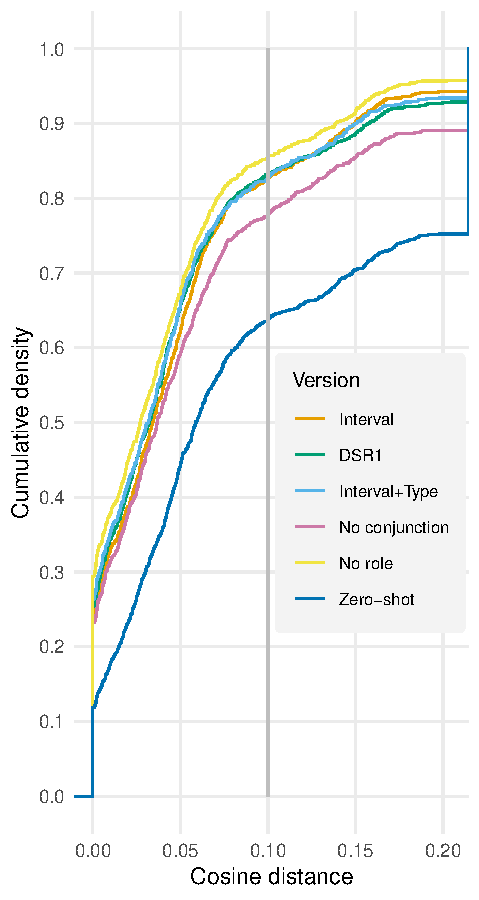
\includegraphics[width=\linewidth]{Plots_tables/prompt_ablation_figure_event_match.pdf}
    \end{minipage}
% \end{figure}
    % \hfill
    \begin{minipage}[t]{0.37\textwidth}
% \begin{figure}[h!]j
    \centering
    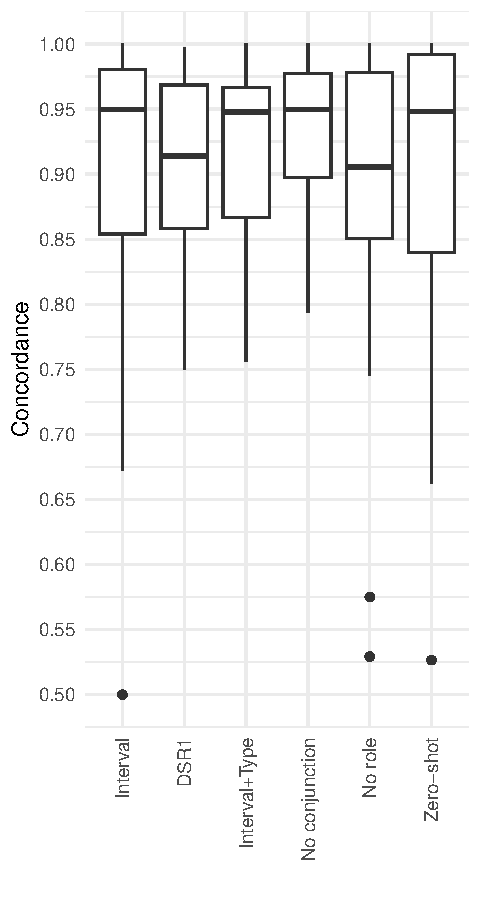
\includegraphics[width=\linewidth]{Plots_tables/prompt_ablation_figure_concordance.pdf}
    \end{minipage}
    % \caption{Event match cumulative distribution function (left) and  concordance box-plots (right) for the sepsis-10 dataset.}
    % \label{fig:sep10eventc}
% \end{figure}
% \begin{figure}[tb!]

    \begin{minipage}[t]{0.35\textwidth}
    \centering
    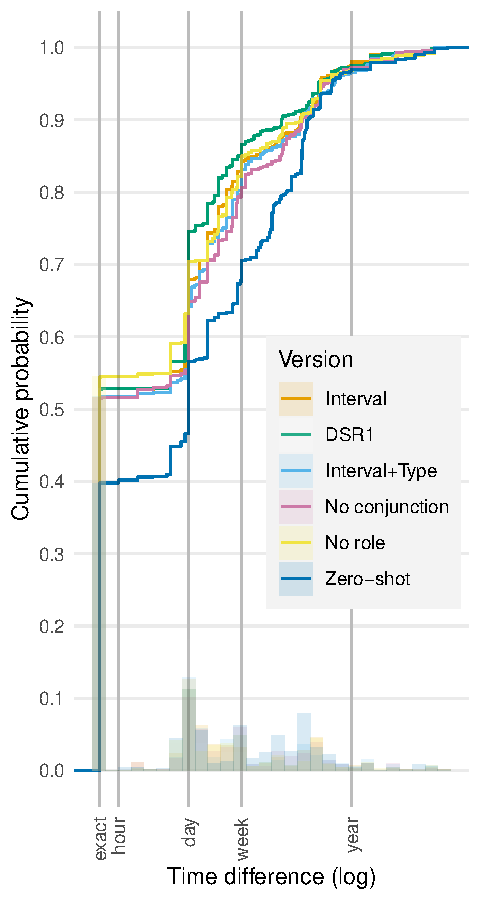
\includegraphics[width=\linewidth]{Plots_tables/prompt_ablation_figure_timediff.pdf}
    \end{minipage}
% \end{figure}
% \begin{figure}[h!]
    \begin{minipage}[t]{0.35\textwidth}
    \centering
    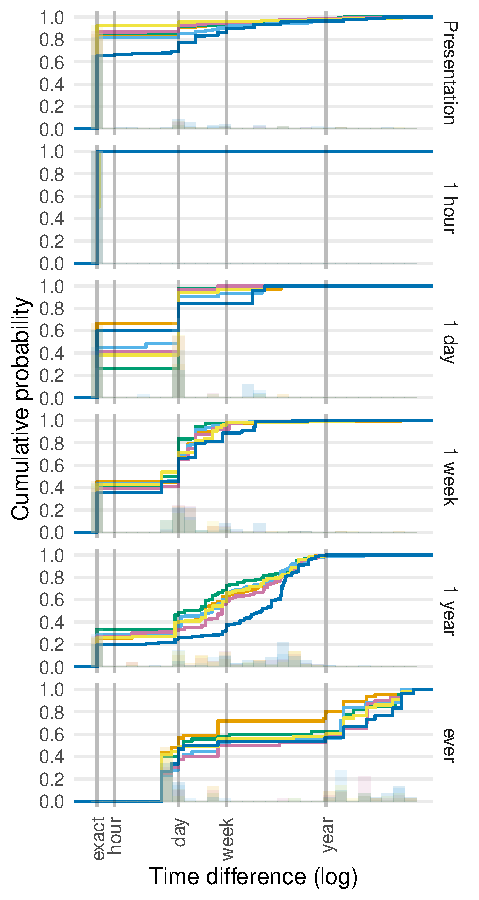
\includegraphics[width=\linewidth]{Plots_tables/prompt_ablation_figure_timediff_subgroup.pdf}
    \end{minipage}
    \caption{Event match cumulative distribution function (left), concordance box plots (middle left), time discrepancy from the manual annotation timestamps among matched events, overall (middle right), and disaggregated by clinician annotator timestamp (time from presentation, right). Each curve represents a different prompt ablation or variant used for extracting temporal clinical events from case reports.}
    \label{fig:prompt_ablation}
    \vspace{-10pt}
\end{figure}

For sensitivity analyses with respect to the quality of different prompt strategies for extracting textual time-series (DeepSeek R1) from PMOA case reports, we omitted selected sections of the LLM query prompt (see Appendix \ref{apd:extraction_prompt} for the full prompt). This led to the following ablations. 

\begin{enumerate}[leftmargin=*,topsep=0pt,itemsep=0pt]
    \item \textbf{No ablation (DSR1)}: Original LLM query prompt for DeepSeek R1.
    
    \item \textbf{No role:} Remove the sentence \texttt{"You are a physician."}
    
    \item \textbf{Zero-shot prompting:} Remove the example case report and textual time-series from the prompt. \\
    %\item \textbf{No conjunction expansion:} 
    \textcolor{teal}{\texttt{An 18-year-old male was admitted to ..}}\\
    "Let's find the locations of event in the case report, it shows that ... then the output should look like:"\\
    \texttt{18 years old | 0 \\
    male | 0 \\
    ..}

    \item \textbf{No conjunction expansion:} Remove the following sentence from the prompt: \texttt{"Separate conjunctive phrases into its component events and assign them the same timestamp (for example, separation of ‘fever and rash’ into 2 events: ‘fever’ and ‘rash’)"}
    
    \item \textbf{Interval:} A query was added to the prompt for extracting the time interval (start and end time of clinical events. The original prompt’s instructions and few-shot examples were modified accordingly. 
    
    \item \textbf{Interval + Type:}. A query was added to the prompt for extracting the ime interval and i2b2
    event type (Interval+Type), where event type is one of: Factual, Possible, Hypothetical, Conditional, Negated, Historical, Uncertain. The original prompt’s instructions and few-shot examples were modified accordingly. 
\end{enumerate}

Figure \ref{fig:prompt_ablation} presents sensitivity analyses for different prompt strategies in extracting structured time-series from clinical narratives. Each ablation tests the effect of removing specific instructional components or adding structured extraction requirements. We evaluate event-level semantic similarity, timestamp accuracy, and temporal concordance across matched events.

\paragraph{Semantic similarity:}
The cumulative density of cosine distances between matched events reveals that omitting key components of the prompt negatively impacts text alignment (Figure Figure \ref{fig:prompt_ablation}, far left). The Interval, DSR1, and Interval+Type prompts consistently show high-quality event matches, with over 80\% of events falling below a cosine distance of 0.1. In contrast, removing role framing (No role) or conjunction splitting (No conjunction) leads to modest degradation. The Zero-shot condition—lacking both examples and guiding instructions—performs markedly worse, with only ~60\% of events under the same similarity threshold.

\paragraph{Temporal concordance:} Concordance index (c-index) measures the agreement between predicted and annotated event ordering (Figure Figure \ref{fig:prompt_ablation}, middle left). The Interval+Type variant achieves the highest median concordance, followed closely by Interval, DSR1, and No role. Removing conjunction expansion reduces ordering consistency slightly, while Zero-shot again yields the lowest performance with a wider spread and multiple outliers (c-index < 0.6), indicating inconsistent temporal sequencing.

\paragraph{Timestamp accuracy:} Cumulative distributions of time discrepancies from manual annotations further support these findings (Figure \ref{fig:prompt_ablation}, middle right). Structured prompts—especially Interval, DSR1, and Interval+Type—demonstrate tighter timestamp alignment. Ablations involving role removal or conjunction omission produce broader error distributions, and Zero-shot extraction results in substantially larger timestamp mismatches.

When stratified by the time from presentation (e.g., within 1 hour, 1 day, 1 week), prompt differences are most pronounced for events occurring farther from the report anchor (Figure \ref{fig:prompt_ablation}, far right). For immediate events, all prompt versions perform comparably. However, at longer timescales (1 week to "ever"), Interval and Interval+Type maintain superior accuracy, while Zero-shot shows dramatic drops in performance. This suggests that structured prompts are particularly critical for accurate long-range temporal reasoning.


%%%%%%%%%%%%%%%%%%%%%%%%%%%%%%%%%%%%%%%%%%%%


% \begin{figure*}[tb!]
%     \begin{minipage}[t]{0.24\textwidth}
%     \centering
%     % \includegraphics[width=\linewidth]{}
%     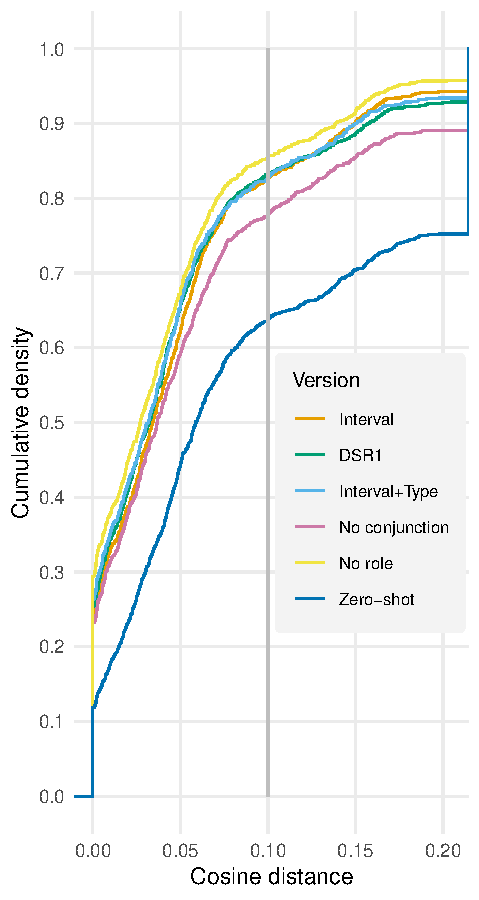
\includegraphics[width=\linewidth]{Plots_tables/prompt_ablation_figure_event_match.pdf}
%     \end{minipage}
% % \end{figure}
%     \hfill
%     \begin{minipage}[t]{0.24\textwidth}
% % \begin{figure}[h!]j
%     \centering
%     % \includegraphics[width=\linewidth]{figures/p25conc.pdf}
%     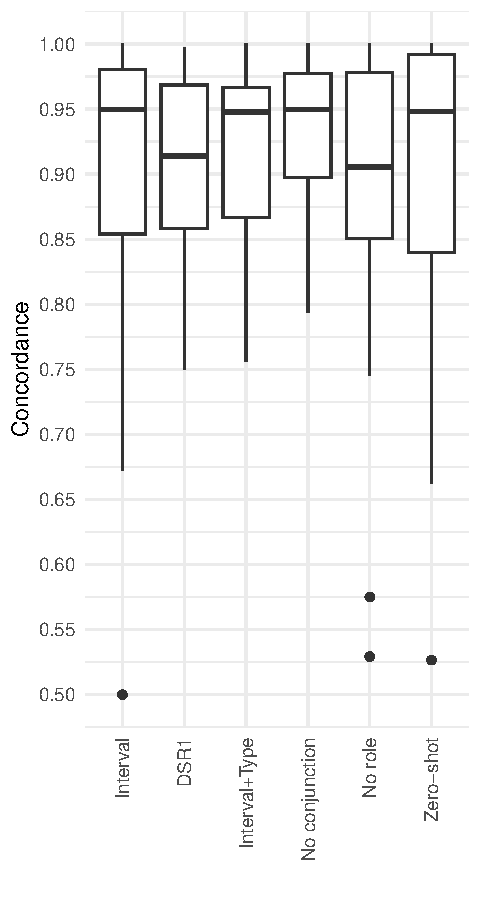
\includegraphics[width=\linewidth]{Plots_tables/prompt_ablation_figure_concordance.pdf}
%     \end{minipage}
%     % \caption{Event match cumulative distribution function (left) and  concordance box-plots (right) for the sepsis-10 dataset.}
%     % \label{fig:sep10eventc}
% % \end{figure}
% % \begin{figure}[tb!]
%     \begin{minipage}[t]{0.24\textwidth}
%     \centering
%     % \includegraphics[width=\linewidth]{figures/p25time.pdf}
%     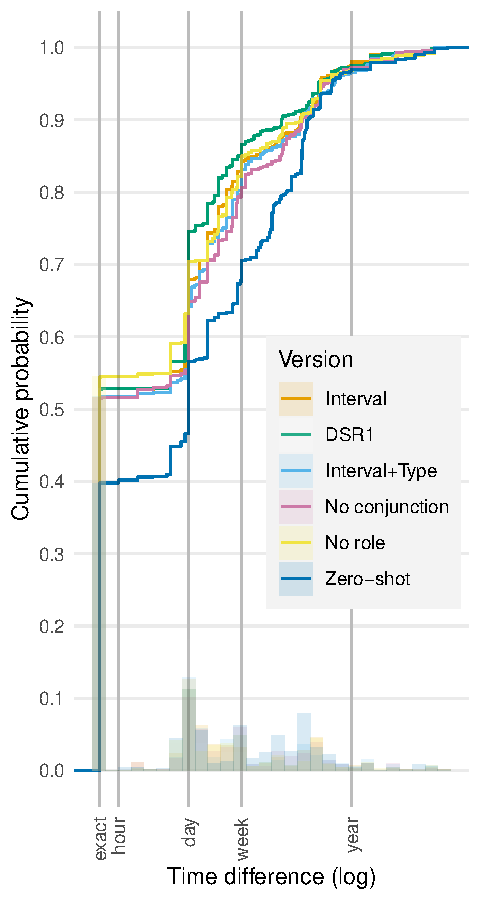
\includegraphics[width=\linewidth]{Plots_tables/prompt_ablation_figure_timediff.pdf}
%     \end{minipage}
% % \end{figure}
% % \begin{figure}[h!]
%     \begin{minipage}[t]{0.24\textwidth}
%     \centering
%     % 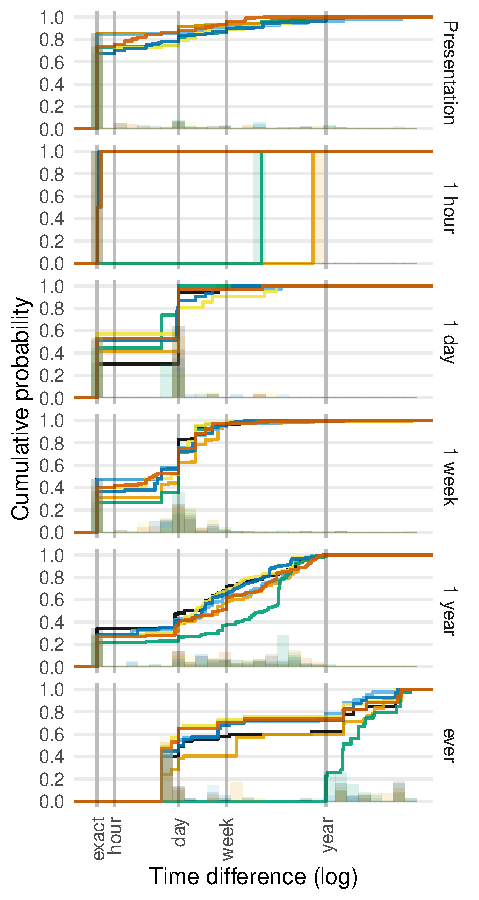
\includegraphics[width=\linewidth]{Plots_tables/pmoa241217_man_o34_figs_Part4.pdf}
%     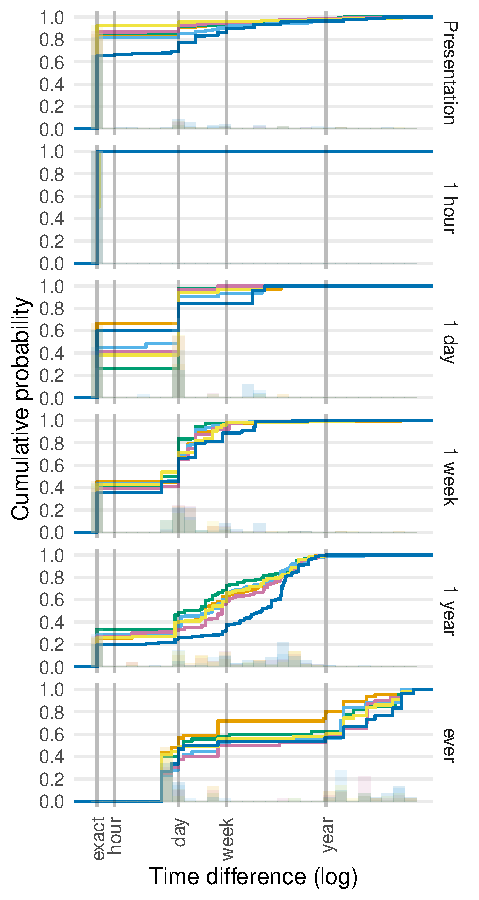
\includegraphics[width=\linewidth]{Plots_tables/prompt_ablation_figure_timediff_subgroup.pdf}
%     \end{minipage}
%     \caption{Event match cumulative distribution function (left), concordance box plots (middle left), time discrepancy from the manual annotation timestamps among matched events, overall (middle right), and disaggregated by clinician annotator timestamp (time from presentation, right). Each curve represents a different prompt ablation or variant used for extracting temporal clinical events from case reports.}
%     \label{fig:prompt_ablation}
%     \vspace{-10pt}
% \end{figure*}


%%%%%%%%%%%%%%%%%%%%%%%%%%%%%%%%%%%%%%%%%%%%%%%%
%%%%%%%%%%%%%%%%%%%%%%%%%%%%%%%%%%%%%%%%%%%%%%%%

\section{Broader Impact}
\label{apd:broader_impact}
% \textcolor{red}{TODO}

The PMOA–TTS corpus contributes to the broader goals of equitable, scalable, and transparent medical AI. However, it also introduces societal considerations related to the use of LLM-generated clinical timelines, especially in sensitive healthcare contexts. Below, we discuss the potential positive and negative societal impacts of our work. 

The PMOA–TTS corpus offers several potential positive contributions to the biomedical NLP and clinical AI communities. By releasing the largest openly available dataset of temporally structured clinical narratives, this work democratizes access to timeline-based clinical text—an area typically limited to proprietary EHR datasets. The corpus spans a wide range of diagnoses and demographics, supporting research on temporal patterns in diverse and sometimes underrepresented conditions. Additionally, by making the extraction pipeline, prompting strategies, and evaluation framework publicly available, the project promotes transparency and reproducibility in LLM-based clinical information extraction. These contributions collectively advance the development of models for timeline reconstruction, temporal reasoning, and longitudinal prediction, while lowering the barrier to entry for researchers working in resource-limited settings.

At the same time, the release and use of PMOA–TTS raise important considerations. Although LLMs achieve strong performance, they may still generate inaccurate or hallucinated outputs, and any downstream use of these annotations without further validation could introduce bias or error. The extraction of structured diagnoses, demographics, and clinical events from public text—though non-identifiable—could also lead to misinterpretation or reinforce historical biases if not handled carefully. Furthermore, while the dataset is intended for research, there is a risk of misapplication in high-stakes clinical settings without expert oversight. Lastly, the stylistic and structural differences between case reports and real-world EHR notes may limit the generalizability of findings derived from PMOA–TTS. These limitations underscore the importance of using the corpus responsibly, with clear reporting of model limitations and appropriate safeguards when applied in downstream tasks.

